\documentclass[a4paper,12pt]{extarticle}

% --- Кодировка и язык ---
\usepackage[utf8]{inputenc}
\usepackage[english,russian]{babel}
\usepackage[T2A]{fontenc}
\usepackage{enumitem}
\usepackage{cmap}

% --- Математика ---
\usepackage[warn]{mathtext}
\usepackage{amsmath,amssymb,mathtools}
\usepackage{multirow}

% --- Графика ---
\usepackage{graphicx}
\usepackage{subcaption}
\usepackage{float}


% --- Отступы и поля (только ОДИН раз!) ---
\usepackage[left=20mm, right=20mm, bottom=20mm, footskip=10mm,
top=20mm, headsep=10mm, headheight=14pt]{geometry}
\usepackage{indentfirst}
\setlength{\parindent}{0.65cm}

\newcommand\Section[1]{
	\refstepcounter{section}
	\section*{\raggedright
		\arabic{section}. #1}
	\addcontentsline{toc}{section}{
		\arabic{section}. #1}
}
\newcommand\Subsection[1]{
	\refstepcounter{subsection}
	\subsection*{\raggedright
		\arabic{section}.\arabic{subsection}. #1}
	\addcontentsline{toc}{subsection}{
		\arabic{section}.\arabic{subsection}. #1}
}
\newcommand\Subsubsection[1]{
	\refstepcounter{subsubsection}
	\subsubsection*{\raggedright
		\arabic{section}.\arabic{subsection}.\arabic{subsubsection}. #1}
	\addcontentsline{toc}{subsubsection}{
		\arabic{section}.\arabic{subsection}.\arabic{subsubsection}. #1}
}

\begin{document}
	
	\begin{titlepage}
		\begin{center}
			{\large МОСКОВСКИЙ ФИЗИКО-ТЕХНИЧЕСКИЙ ИНСТИТУТ (НАЦИОНАЛЬНЫЙ ИССЛЕДОВАТЕЛЬСКИЙ УНИВЕРСИТЕТ)}
		\end{center}
		\begin{center}
			{\large{Физтех-школа электроники, фотоники и молекулярной физики}}
		\end{center}
		
		\vspace{7cm}
		
		{\huge
			\begin{center}
				{Лабораторная работа}\\
				{\bf Строки }\\
				{Кривопалова Полина Б04-501}\\
			\end{center}
		}
		\vspace{6cm}
		
		\vspace{5.5cm}
		\begin{center}
			Долгопрудный, ноябрь 2026
		\end{center}
	\end{titlepage}
	
	\Section{Исследование времени работы}
	\Subsection{Опыт А}
	\subsubsection*{Предположение}
	
	При работе с скалярной величиной время обращения будет минимальным и не зависит от типа обращения. \\
	Обращение к Text будет быстрее, чем к Block и в обоих случаях время обращения по значению будет наибольшим, по ссылке и указателю одинаковым. От размера структур не зависит.\\
	При включении оптимизаций время уменьшится на пару порядков
	
	\subsubsection*{Методика}
	
	Измерения проводились при помощи функций аналогичных представленной
	
	\begin{figure}[h!] 
		\centering
		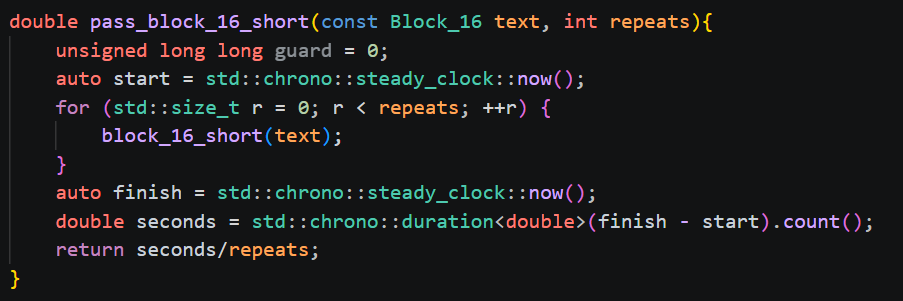
\includegraphics[width=0.7\textwidth]{method1.png}
		\label{fig:model1}
	\end{figure}
	
	\subsubsection*{Результаты}
	
	\begin{figure}[h!] 
		\centering
		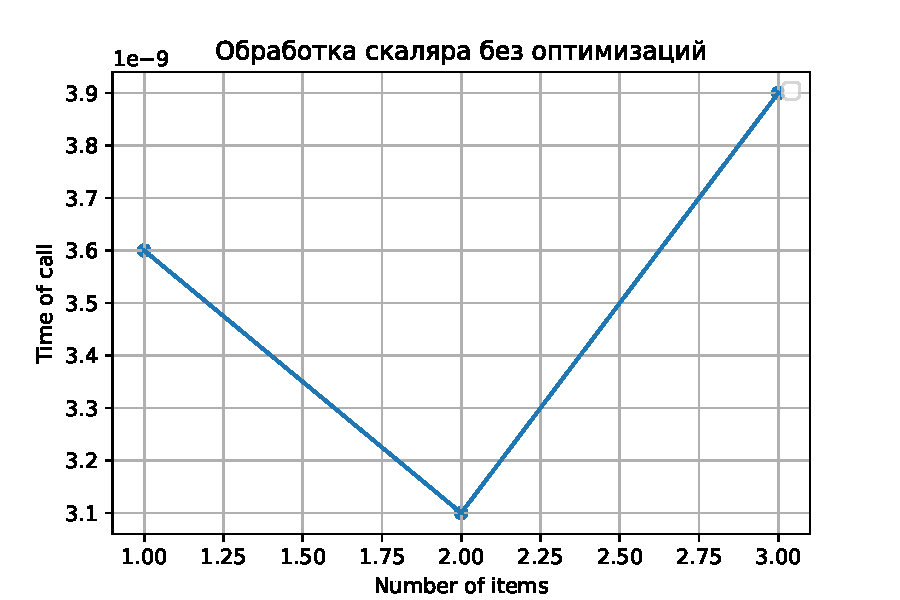
\includegraphics[width=0.7\textwidth]{Scalar.pdf}
		\label{fig:scalar}
	\end{figure}
	
	
	\begin{table}[H]
		\centering
		\begin{tabular}{cc}
			\begin{subfigure}{0.5\textwidth}
				\centering
				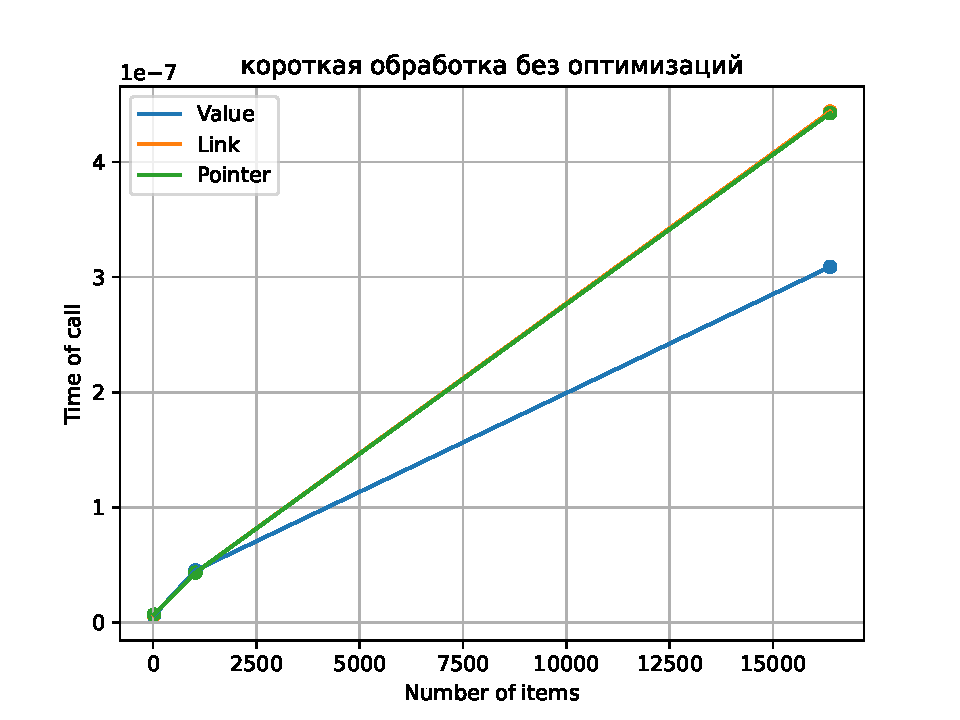
\includegraphics[width=\columnwidth]{Block_short.pdf}
			\end{subfigure} &
			\begin{subfigure}{0.5\textwidth}
				\centering
				\includegraphics[width=\columnwidth]{Text_short.pdf}
			\end{subfigure} \\
			\newline
			\begin{subfigure}{0.5\textwidth}
				\centering
				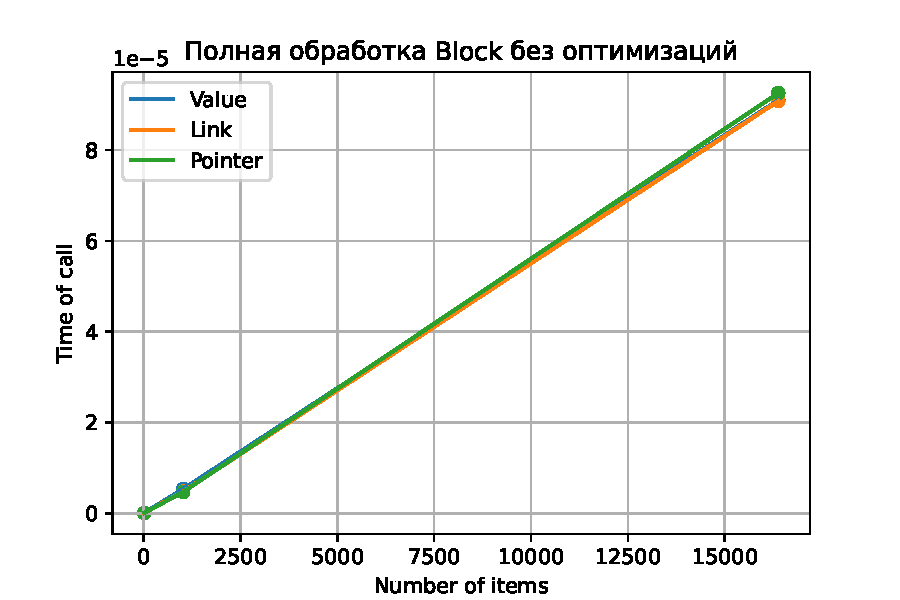
\includegraphics[width=\columnwidth]{Block_full.pdf}
			\end{subfigure} &
			\begin{subfigure}{0.5\textwidth}
				\centering
				\includegraphics[width=\columnwidth]{Text_full.pdf}
			\end{subfigure} \\
		\end{tabular}
		\label{tab:call}
	\end{table}
	
	\begin{figure}[h!] 
		\centering
		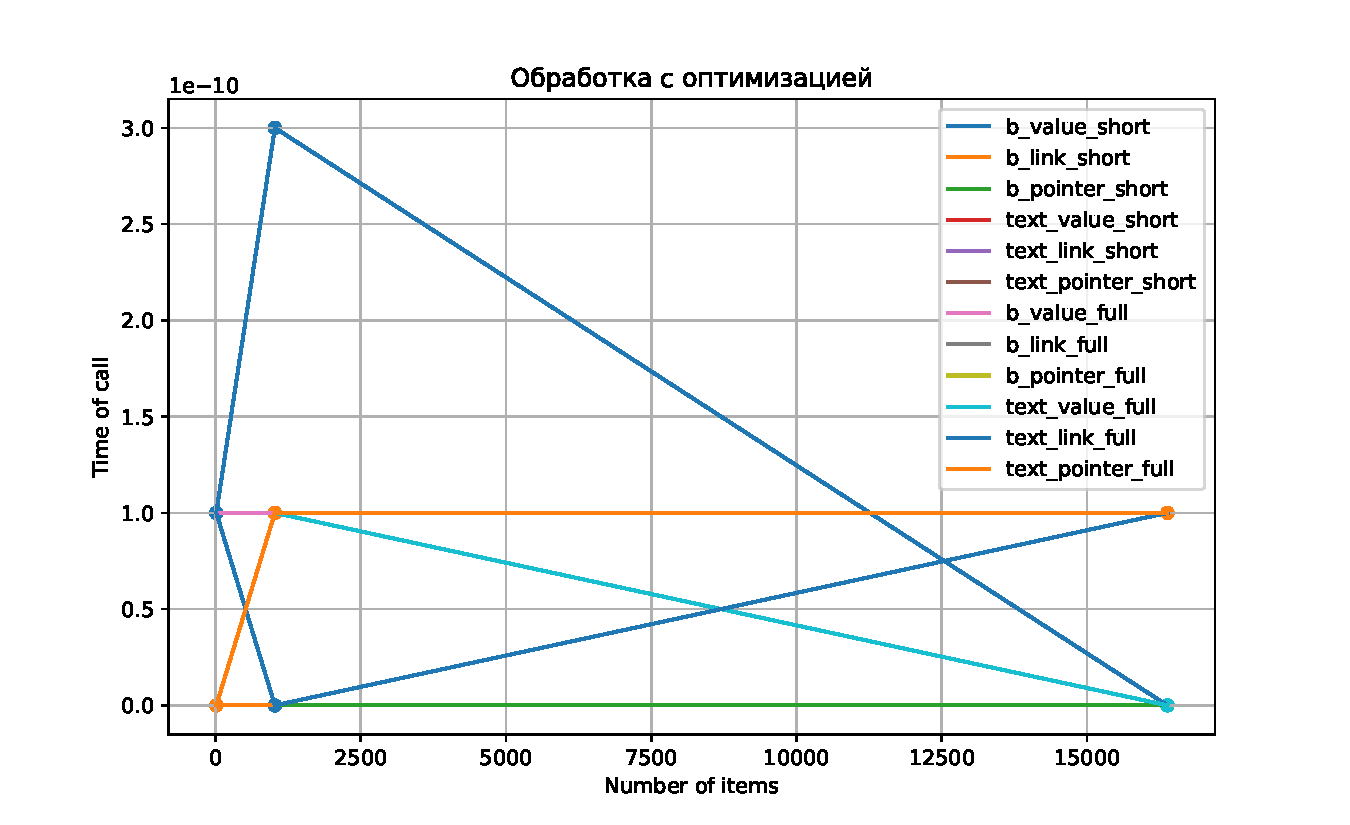
\includegraphics[width=0.7\textwidth]{O2.pdf}
		\label{fig:O2}
	\end{figure}
	
	\subsubsection*{Объяснение результатов}
	
	Для скаляра данные похожи больше на случайные выбросы.\\
	При коротком варианте обращение по значению наиболее бстрое для обоих структур. Это может быть связано с тем, что когда передаётся ссылка и указатель происходит дополнительный шаг расшифровки, что замедляет работу.\\
	При полной обработке для Block разницы нет. А для Text наоборот: при обрашении по значению время наибольшее. Причиной может быть то, что \\
	Разброс значений при оптимизации скорее случайный, чем показательный
	
	\Subsection{Опыт В}
	
	\subsubsection*{Предположение}
	
	При анализировании исходного текста время будет минимальным. Многократное копирование будет самым долгим. Эта тенденция будет наблюдаться при обоих параметрах сравнения.
	
	\subsubsection*{Методика}
	
	Измерения проводились при помощи функций аналогичных представленной
	
	\begin{figure}[h!] 
		\centering
		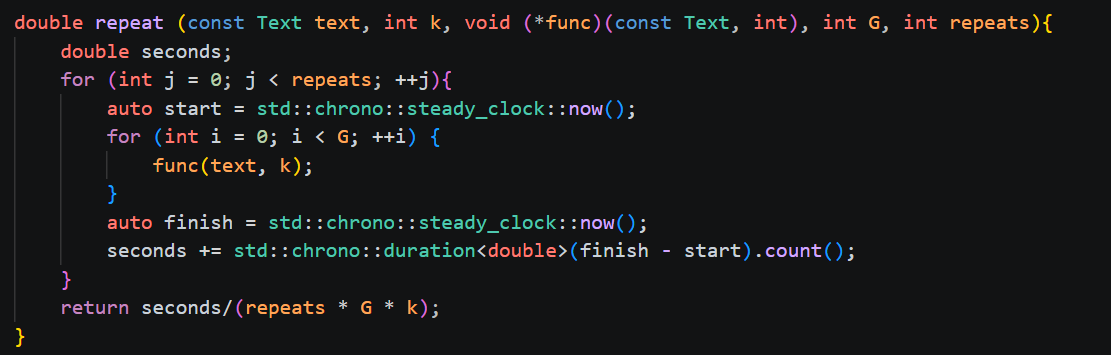
\includegraphics[width=0.7\textwidth]{method2.png}
		\label{fig:model2}
	\end{figure}
	
	\subsubsection*{Результаты}
	
	\begin{table}[H]
		\centering
		\begin{tabular}{cc}
			\begin{subfigure}{0.5\textwidth}
				\centering
				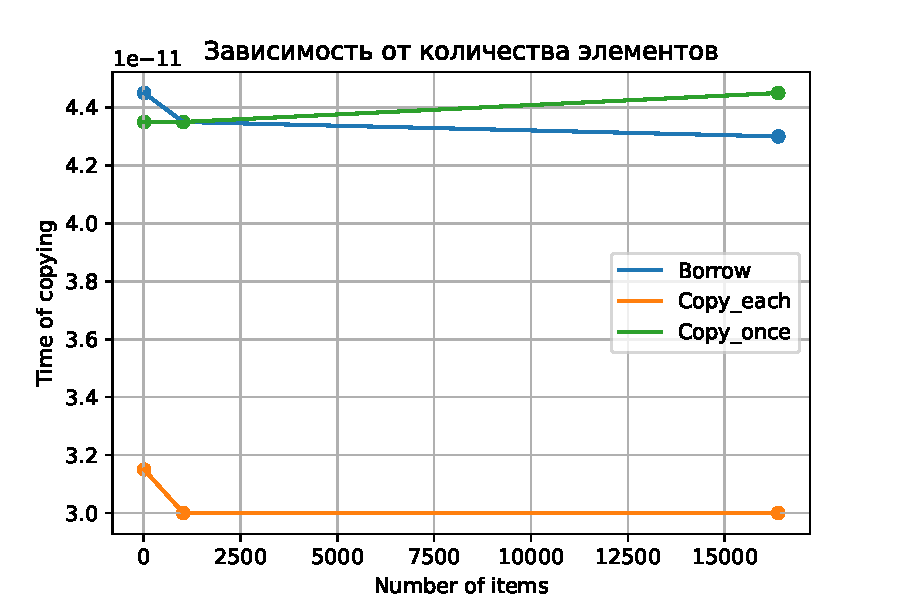
\includegraphics[width=\columnwidth]{Items_copy.pdf}
			\end{subfigure} &
			\begin{subfigure}{0.5\textwidth}
				\centering
				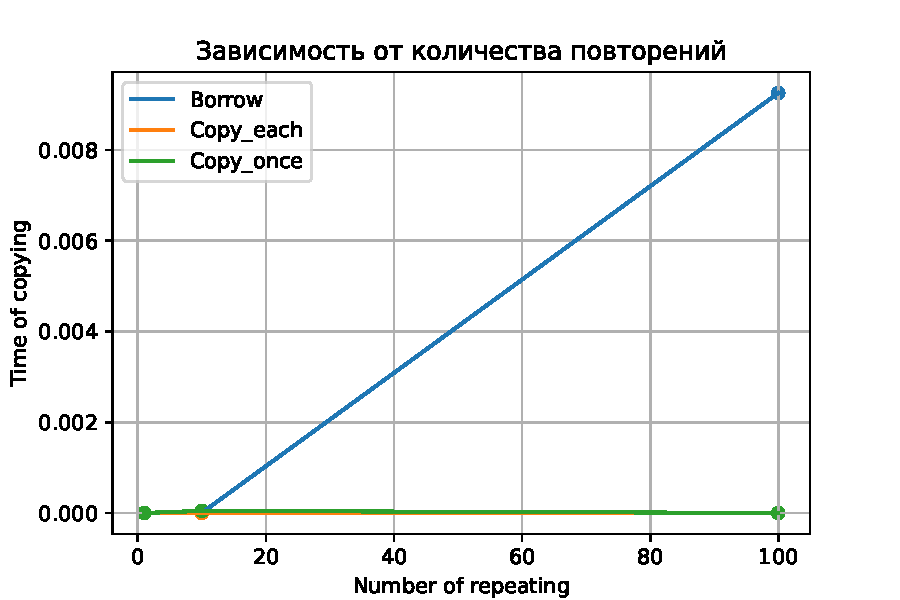
\includegraphics[width=\columnwidth]{Repeating_copy.pdf}
			\end{subfigure} \\
		\end{tabular}
		\label{tab:copy}
	\end{table}
	
	\subsubsection*{Объяснение результатов}
	
	\Section{Исследование работы с памятью}
	\subsection*{Предположение}
	\subsection*{Методика}
	\subsection*{Результаты}
	
	\begin{table}[h]
		\centering
		\label{tab:results}
		\begin{tabular}{|r|l|r|r|r|r|r|}
			\hline
			\textbf{length} & \textbf{mode} & \textbf{repeats} & \textbf{uses} & \textbf{allocations} & \textbf{copied\_bytes} & \textbf{extra\_bytes} \\
			\hline
			15     & borrow     & k=1 G=100      & 1   & 0     & 0         & 0     \\
			1023   & borrow     & k=1 G=100      & 1   & 0     & 0         & 0     \\
			16383  & borrow     & k=1 G=100      & 1   & 0     & 0         & 0     \\
			15     & copy\_each & k=1 G=100      & 1   & 100   & 1500      & 16    \\
			1023   & copy\_each & k=1 G=100      & 1   & 100   & 102300    & 1024  \\
			16383  & copy\_each & k=1 G=100      & 1   & 100   & 1638300   & 16384 \\
			15     & copy\_once & k=1 G=100      & 1   & 100   & 1500      & 16    \\
			1023   & copy\_once & k=1 G=100      & 1   & 100   & 102300    & 1024  \\
			16383  & copy\_once & k=1 G=100      & 1   & 100   & 1638300   & 16384 \\
			\hline
			15     & borrow     & k=10 G=100     & 10  & 0     & 0         & 0     \\
			1023   & borrow     & k=10 G=100     & 10  & 0     & 0         & 0     \\
			16383  & borrow     & k=10 G=100     & 10  & 0     & 0         & 0     \\
			15     & copy\_each & k=10 G=100     & 10  & 1000  & 15000     & 16    \\
			1023   & copy\_each & k=10 G=100     & 10  & 1000  & 1023000   & 1024  \\
			16383  & copy\_each & k=10 G=100     & 10  & 1000  & 16383000  & 16384 \\
			15     & copy\_once & k=10 G=100     & 10  & 100   & 1500      & 16    \\
			1023   & copy\_once & k=10 G=100     & 10  & 100   & 102300    & 1024  \\
			16383  & copy\_once & k=10 G=100     & 10  & 100   & 1638300   & 16384 \\
			\hline
			15     & borrow     & k=100 G=100    & 100 & 0     & 0         & 0     \\
			1023   & borrow     & k=100 G=100    & 100 & 0     & 0         & 0     \\
			16383  & borrow     & k=100 G=100    & 100 & 0     & 0         & 0     \\
			15     & copy\_each & k=100 G=100    & 100 & 10000 & 150000    & 16    \\
			1023   & copy\_each & k=100 G=100    & 100 & 10000 & 10230000  & 1024  \\
			16383  & copy\_each & k=100 G=100    & 100 & 10000 & 163830000 & 16384 \\
			15     & copy\_once & k=100 G=100    & 100 & 100  & 1500      & 16    \\
			1023   & copy\_once & k=100 G=100    & 100 & 100  & 102300    & 1024  \\
			16383  & copy\_once & k=100 G=100    & 100 & 100  & 1638300   & 16384 \\
			\hline
		\end{tabular}
		\caption{Результаты работы с памятью}
	\end{table}
	
	\subsection*{Объяснение результатов}
	Все предположения оказались верными
\end{document}